\documentclass[runningheads]{llncs}
%---- Sonderzeichen-------%
\usepackage[ngerman]{babel}
%---- Codierung----%
\usepackage[utf8]{inputenc}
%\usepackage[latin1]{inputenc}
\usepackage[T1]{fontenc}
\usepackage{graphicx}
\usepackage{url}
\usepackage{llncsdoc}
%----- Mathematischer Zeichenvorrat---%
\usepackage{amsmath}
\usepackage{amssymb}
\usepackage{enumerate}
% fuer die aktuelle Zeit
\usepackage{listings}
\usepackage{subfigure}
\usepackage{hyperref}
\renewcommand{\labelitemi}{$\bullet$}

\setcounter{tocdepth}{3}
\setcounter{secnumdepth}{3}

% -------------------------------------------------------------------------------------------------
% -------------------------------------------------------------------------------------------------
\mainmatter
\title{Universal Rendering}
\titlerunning{Universal Rendering}
\author{Julian Beck}
\authorrunning{Julian Beck}
\institute{Betreuer: Prof. Dr. rer. nat. Christian Zirpins}
\date{01.05.2019}
\begin{document}
\let\oldaddcontentsline\addcontentsline
\def\addcontentsline#1#2#3{}
\maketitle
\def\addcontentsline#1#2#3{\oldaddcontentsline{#1}{#2}{#3}}

% -------------------------------------------------------------------------------------------------

\begin{abstract}
  An dieser Stelle sollte später eine Kurzzusammenfassung stehen.
\end{abstract}

% -------------------------------------------------------------------------------------------------
\tableofcontents 
\newpage
% -------------------------------------------------------------------------------------------------

\section{Einleitung}
\label{sec:Einleitung}
Seit dem Beginn des Webs funktioniert das Surfen wie folgt: 
Ein Webbrowser fordert eine bestimmte Seite an, ein Server im 
Internet bearbeitet die Anfrage und generiert ein HTML 
(Hypertext Markup Language) Dokument als Antwort. 
Dies bezeichnet man als serverseitiges rendern. 
In den Anfängen des Webs stellte dies kein Problem dar, 
da die Browser nicht leistungsstark waren und die Webseiten 
aus meist statischen Inhalt bestanden. 
Später mit HTML5 wurden Webseiten dynamischer und 
interaktiver für den Nutzer, was dazu führte, dass immer mehr Apps, 
sogenannte Single Page Applikationen, 
vollständig im Browser auf einer Seite liefen. 
Um dies zu ermöglichen wird clientseitiges rendern verwendet. 
Single Page Applications oder kurz SPAs, bieten Vorteile für den Anwender: 
Sie reagieren schnell auf Benutzerinteraktionen und können zwischen Seiten navigieren, 
ohne sie komplett neu zu laden. Gleichzeitig sind SPAs komfortabel zu entwickeln, 
dank moderner Frameworks. Beide Varianten, serverseitiges und clientseitiges rendern, 
haben Vor- und Nachteile. Universal Rendering kombiniert die beiden Ansätze und 
erfüllt alle Anforderungen an eine moderne Webanwendung.



\subsection{Anforderungen an eine Webanwendung}
\label{subsec:Anforderungen an eine Webanwendung}

Eine moderne Webanwendungen sollten folgende Anforderungen erfüllen\cite{IsomorphicApps}:
\begin{itemize}
  \setlength\itemsep{1em}
  \item Damit die Seite von Suchmaschinen gefunden werden kann, sollte sie von Suchmaschinen Crawler indexierbar sein. 
  Dies wird Suchmaschinenoptimierung oder auch SEO 
  (engl. search engine optimization) genannt. 
  \item Eine moderne Webseite muss beim Aufrufen für den Anwender schnell laden. Der Anwender sollte nicht lange warten 
  müssen bis er die Anwendung sieht und mit ihr interagieren kann
  \item Eine moderne Webanwendung muss dynamisch und interaktiv sein. Die Anwendung sollte auf Benutzereingaben reagieren, 
  ohne lange Ladezeiten oder neuladen der Seite.
  Die Anwendung sollte einfach zu entwickeln sein und gleichzeitig muss sichergestellt werden, 
  dass der Programmcode einfach zu pflegen ist. 
  Code duplikation sollte minimiert werden.
\end{itemize}

\subsection{Terminologie}
\label{subsec:Terminologie}
Beim Rendern in der Webtechtechnologie Unterscheidet man zwischen 
zwei verschiedenen Arten des Renderns:
\begin{itemize}
  \setlength\itemsep{1em}
  \item Im allgemeinen Sprachgebrauch versteht man unter dem
  Begriff des Renderns, das Abbilden von Informationen für eine von dem Benutzer
  wahrnehmbare Art, meistens in visueller Form. Für Webseiten findet dieses Rendern 
  immer auf der Clientseite, also im Browser statt. Der Browser verfügt über eine rendering Engine,
  die das darzustellene HTML Dokument als Document Object Model (DOM) und CSS Object Model (CSSOM) parst.
  Anschließend wird die Seite von dem Browser gezeichnet und dargestellt.\cite{chen_geroimenko_2006}
  \item Das generieren von HTML Dokumenten wird in der Webtechnologie auch als Rendern 
  bezeichnet. Ruft man beispielsweise eine Webseite auf und es wird ein HTML Dokument für diese 
  Anfrage generiert, bezeichnet man dies auch als Rendern. Dieser Vorgang kann im Gegensatz zum visuellen Rendern,
  auf der Client- oder Serverseite stattfinden.
\end{itemize}
Der Begriff Universal Rendering beschreibt eine Kombination aus server- und clientseitiges rendern. 
Dieser Ansatz wird oft auch als Isomorphic oder Server-Side Rendering bezeichnet.
Folgende Begriffe beschreiben unterschiedliche Zeiten beim Laden einer Webseite:
\begin{itemize}
  \setlength\itemsep{1em}
  \item \textbf{TTFB}: Time to First Byte - Zeit bis zum ersten Byte -  Die Zeit zwischen dem Klicken auf ein Link und Erhalten der Daten vom Server.
  \item \textbf{FP}: First Paint - der Zeitpunkt an dem der erste Inhalt für den User sichtbar wird.
  \item \textbf{FCP}: First Contentful Paint oder auch First Meaningful Paint - Der Zeitpunkt, an dem der Benutzer den wichtigsten Inhalt einer Website als fertig geladen sieht. Die Zeit bis zum FCP wird auch als kritischer Rendering-Pfad (engl.:Critical Rendering Path) bezeichnet.
  \item \textbf{TTI}: Time To Interactive - Die Zeit bis die Seite interaktiv wird und der Anwender mit ihr interagieren kann.
\end{itemize}
Da die Anwendung vollständig auf der Client Seite läuft, ist es schwierig für Suchmaschinen Crawler die seite zu Indexieren was zu einer schlechten SEO führt.
Des weiteren, dadurch dass die Webseite nicht auf dem Server, sonder vom Client gerendert wird, muss der User warten bis die seite vollständig gerendert wird.
Server Side rendering ist eine Mischung beider Ansätze. Es kombiniert die SEO und Performance von Server seitigen Applikationen und die Interaktivität und flexibilität von Client Side Anwendungen.
\\
\\
Diese Arbeit beginnt mit den der Funktionsweise von server - und clientseitigen Rendern. 
Es werden die Vor - und Nachteile der jeweiligen Vorgehensweisen untersucht 
und beschrieben warum eine Notwendigkeit für Universal Rendering besteht. Nach einer Einführung in den Universal Rendering Vorgang, werden die verwendeten Technologien und deren Funktionsweise für das Rendern beschrieben. Anschließend werden die positiven und negativen Aspekte des Universal Rendering beschrieben und Alternativen genannt. Danach beschreibt die Arbeit unterschiedliche Frameworks zum implementieren der Rendering Technologie und zeigt wie Unternehmen Universal Rendering verwenden. Das Fazit erarbeitet wann welche Rendering Technologie verwendet werden soll und zeigt den aktuellen Stand von Suchmaschinen Crawler.
\newpage
% -------------------------------------------------------------------------------------------------

\section{Serverseitiges Rendering - SSR}
\label{sec:Serverseitiges Rendering}
Bei der klassische Web-Architektur oder auch \textit{Thin Client - Fat Server”} 
Architektur, befindet sich die Anwendungslogik auf der Serverseite. 
Diese Logik wird durch Programmiersprachen wie PHP, Python oder Java 
implementiert. Die Clientseite ist nur zuständig für die Document Object Model 
Manipulation und dem Darstellen der Webseite im Browser. Abbildung \ref{Thin Client - Fat Server Architektur einer SSR Anwendung} 
zeuigt den Aufbau einer SSR Anwendung. Die Datenbankschicht ist zuständig für das Komunizieren mit einer exteren
Datenbank, die Anwendungsschicht verarbeitet die Anfrange und beinhaltet die eigentliche Logik und die Präsentationsschicht generiert,
das sogennante rendern, das HTML Dokument. \cite{IsomorphicApps} \cite{subramanian}
\begin{figure}[h]
  \centering
  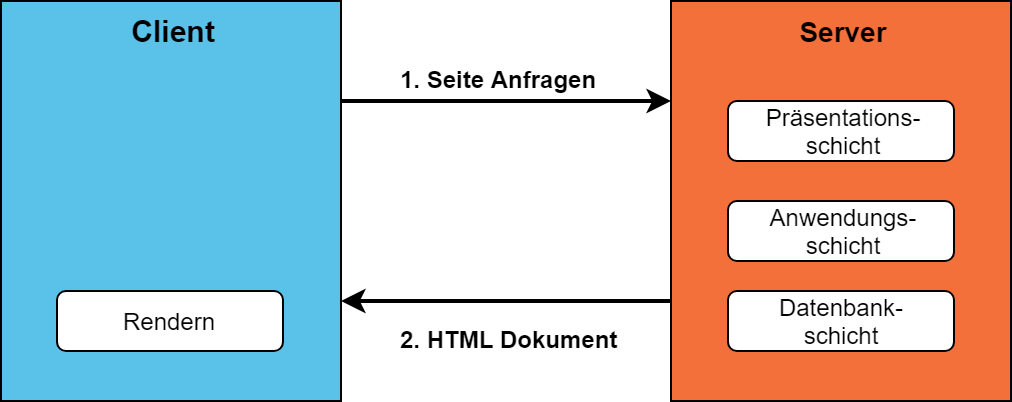
\includegraphics[width=12cm]{images/server}
  \caption{Thin Client - Fat Server Architektur einer SSR Anwendung}
  \label{Thin Client - Fat Server Architektur einer SSR Anwendung}
\end{figure}
\\
Wird eine Website aufgerufen, wird zunächst über das HTTP Protokoll 
eine GET Anfrage an den Server gesendet. Dieser bearbeitet die Anfrage 
und antwortet mit einem HTML Dokument. Auf der Clientseite wird das HTML 
von dem Browser interpretiert und dargestellt.
\\
\\
Der kritische Rendering-Pfad ist bei klassischen Webanwendungen sehr schnell, 
da das HTML vom Server gerendert wird. Dies bietet eine gute Nutzererfahrung, 
da der Client ausschließlich die Webseite als DOM darzustellen muss. 
Beim Erhalten der Antwort, sieht der Anwender schon den First Contentful Paint 
und kann mit der Seite interagieren. Damit ist die Zeit bis zum FCP gleich lang, 
wie die Time to Interactive der Website. Dies bringt eine gute Nutzererfahrung, 
da der User sofort nach dem Laden mit der Website interagieren kann, 
anders als bei Clientseitigen Anwendungen. 
Da die Webseite direkt mit HTML antwortet, ist es einfach für Suchmaschinen Crawler 
die Webseite zu indexieren. 
\\
\\
Der entscheidende Nachteil von klassischen serverseitigen Anwendungen 
ist die Benutzer Interaktivität. Für jede Navigation zwischen verschiedenen 
Seiten und für jedes abgeschickte HTML-Form, 
muss eine neue Anfrage an den Server gesendet werden. 
Dies erfordert ein komplettes Neuladen der Webseite, 
auch wenn nur ein einziges Element aktualisiert werden soll. 
Da der Browser bei auf diese Art nur eine Anfrage bearbeiten kann, 
bezeichnet man dies als synchrone Kommunikation. 
Mit dem Einführen von Ajax wurden Webanwendungen asynchron, 
was zu einer besseren Nutzererfahrung führte.

\subsection{Serverseitiges Rendering mit Ajax}
\label{subsec:Serverseitiges Rendering mit Ajax}
Mit der Einführung von XMLHttpRequest von Microsoft im Jahre 2000 wurde die Basis von Ajax geschaffen. 
Ajax oder auch “asynchronous JavaScript and XML” erlaubt eine asynchrone Datenübertragung mit dem Server.
\\
\\
Ajax löst das Problem der synchronen Kommunikation klassischer Webanwendungen. 
Ajax ermöglicht es asynchron, 
den Inhalt einer Webseite zu aktualisieren und Daten zum Server senden und empfangen, 
ohne neuladen der Webseite. Damit dies möglich ist, 
kommuniziert die Clientseite, mittels Ajax, mit dem Server. 
So ist es möglich, interaktive und dynamische Webanwendungen zu bauen, 
die sofort reagieren ohne ein Neuladen der Seite. \cite{IsomorphicApps}
\begin{figure}[h]
  \centering
  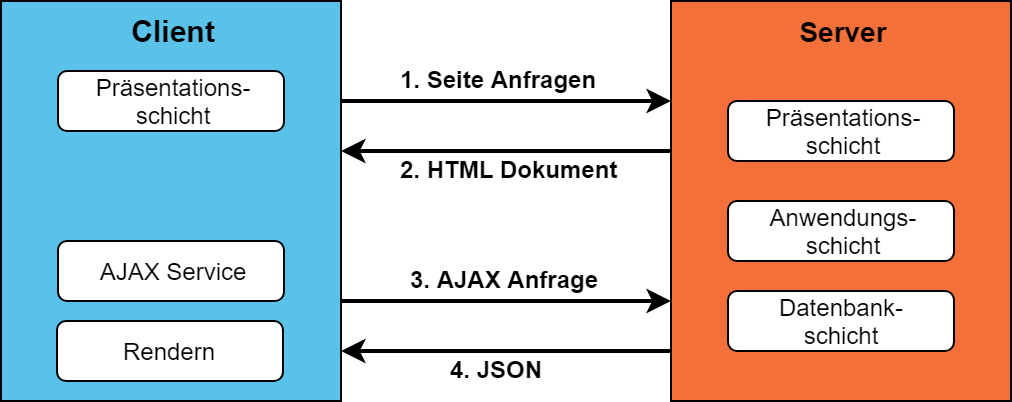
\includegraphics[width=12cm]{images/serverajax}
  \caption{SSR Architektur mit Ajax}
  \label{SSR Architektur mit Ajax}
\end{figure}
\\
Die Verwendung von Ajax führt aber auch zu einer komplizierten Web-Architektur. 
Zuvor war die Anwendungslogik auf der Serverseite. 
Dies erlaubte eine klare Trennung zwischen Client und Server. 
Das Aktualisieren von Teilbereichen der Webseite führt 
zu einer Verbesserung der Nutzererfahrung. 
Es erfordert aber auch doppelte Templates und erhöht den Programmanteil sowie Logik auf der Clientseite.

Um Ajax zu benutzen ist mehr JavaScript auf der Clientseite erforderlich. 
Besitzt eine Anwendung Logik auf der Client- und Serverseite, 
wird es schwerer diese zu entwickeln. 
ie Wartbarkeit wird erhöht und es sind mehr Unittests nötig, 
die sicherstellen, dass der Zustand der Anwendung auf Server und 
Client gleich ist. 
\newpage
% -------------------------------------------------------------------------------------------------

\section{Clientseitiges Rendering - CSR}
\label{sec:Clientseitiges Rendering}
Single Page Application kurz SPAs werden durch moderne Frameworks wie \textit{React}, 
Vue und \textit{Angular} immer beliebter. SPAs sind komfortabel zu Entwickeln 
und lösen das Problem der Wartbarkeit, 
indem sie vollständig auf der Clientseite, 
im Browser, ausgeführt werden.
\\
\\
Single Page Application verwenden die \textit{Fat- Client, Thin Server Architektur}. 
Dabei befindet sich die Anwendungs- und Interface Logik vollständig auf der Clientseite, wie Abbildung 
\ref{Fat Client - Thin Server Architektur einer CSR Anwendung} zeigt.
Die Serverseite ist nur zuständig für das Bereitstellen von Anwendungsdaten 
und benötigten Scripts. 
Beim Aufrufen einer Single Page Application antwortet der Server 
mit einem leeren HTML Dokument, das nur ein Template und Links 
zu den benötigten Scripts enthält. 
Der Client lädt anschließend die JavaScript Dateien runter, 
initialisiert die Anwendung und rendert das HTML im Browser. 
Damit findet das Rendern der Anwendung nur auf der Clientseite statt. 
Ist der Client initialisiert, ruft er mittels Ajax weitere Anwendungsdaten ab. 
\begin{figure}[h]
  \centering
  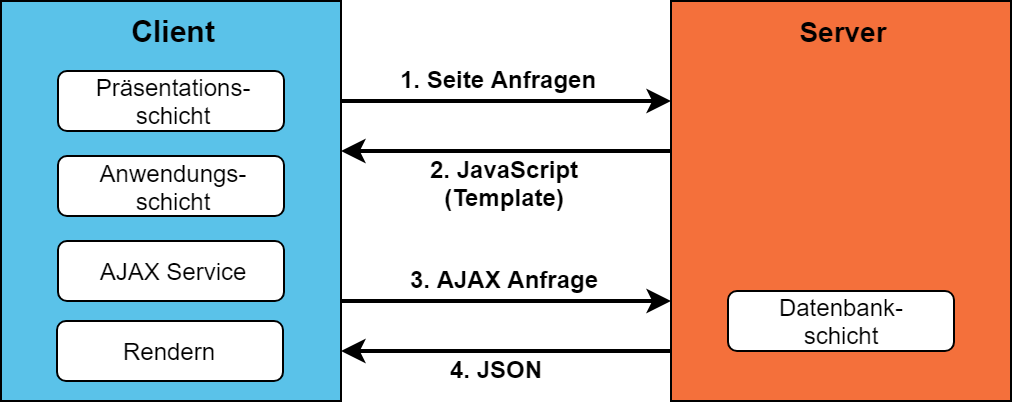
\includegraphics[width=12cm]{images/client}
  \caption{Fat Client - Thin Server Architektur einer CSR Anwendung}
  \label{Fat Client - Thin Server Architektur einer CSR Anwendung}
\end{figure}
\\
Dieses Vorgehen hat Vorteile beim Wechseln zwischen einzelnen Seiten. 
Der Client muss beim Navigieren keine neue Daten vom Server anfordern, 
sondern nur den angezeigten Inhalt wechseln. 
Somit ist kein Neuladen der Seite nötig. 
Aus diesem Grund werden Single Page Apps oft bei interaktiven Anwendung, 
wie beispielsweise Googles GMAIL verwendet. 
Da die Anwendungslogik vollständig auf der Clientseite liegt, 
ist eine klare Trennung zwischen Server und Client möglich. 
Dies vereinfacht das Entwickeln von SPAs und
macht in Kombination mit modernen Frameworks 
Single Page Applications bei Entwicklern sehr beliebt.
\\
\\
Beim Aufrufen von serverseitig gerenderten Webseiten antwortet
der Server direkt mit einem HTML Dokument, 
dass den angeforderten Inhalt enthält. 
Bei SPAs hingegen antwortet der Server nur mit einem Template. 
Der Client lädt anschließend die JavaScript Bibliotheken, 
wie beispielsweise \textit{React} und initialisiert die Webseite. 
Während dem Initialisieren kann der Anwender nicht mit der Seite interagieren
und muss warten. Oft werden Ladebalken verwendet, 
die der Benutzer sieht, bis die Seite geladen ist. 
Aus diesem Grund ist die Time to Interactive und 
der kritische Rendering-Pfad sehr hoch, im Gegensatz zu SSR. 
\\
\\
Ein weiteres Problem mit SPAs ist die Search Engine Optimization (SEO). 
Da beim Aufrufen einer CSR Anwendung der Server nur mit einem Template 
antwortet, dass nur JavaScript und kein Inhalt enthält, 
kann es nicht von Suchmaschinen indexiert werden. 
Beim Indexieren einer \textit{React} Anwendung beispielsweise, 
enthält der Crawler die in Abbildung \ref{HTML Antwort einer Single Page React Anwendung} enthaltene Antwort des Servers. 
Die Antwort enthält im Body des HTML Dokuments nur ein ROOT Element und Links zu
den benötigten JavaScript Datein. Nach dem Laden und Initalisieren des clientseitigen Frameworks,
started das Framework im ROOT Element der Anwendung
\begin{figure}[h]
  \centering
  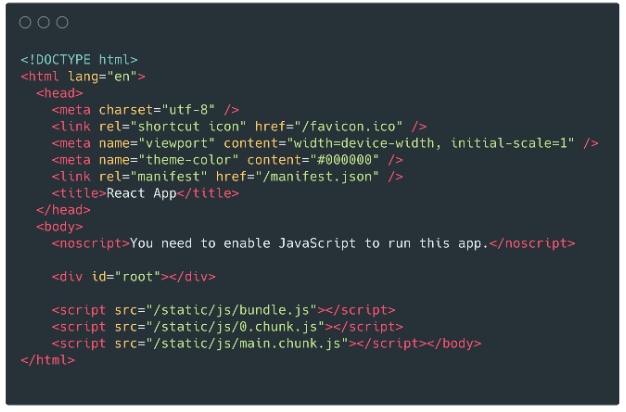
\includegraphics[width=12cm]{images/react-code-small}
  \caption{HTML Antwort einer Single Page \textit{React} Anwendung}
  \label{HTML Antwort einer Single Page React Anwendung}
\end{figure}
\\
Damit ein Suchmaschienprovider eine Single Page Anwendung indexieren kann,
muss er die Seite rendern,
was nicht jeder Suchmaschinen Provider macht. 
Eine weitere Herausforderung bei der SEO sind die URLs der Anwendung. 
SPAs verwenden Hash Marks zur Navigation zwischen Seiten. 
Eine Hash Mark wird am Ende einer SPA Domain verwendet. 
Zum Beispiel würde aus einer der URL \url{https://example/test} bei einer SPA 
\url{https://example#/test} werden. 
Das Verwenden des Hash am Ende der URL verhindert, 
dass der Browser eine neue Anfrage sendet. 
Dies ist wichtig, da die Grundidee einer SPA darin besteht, 
dass nur die Daten angefordert werden, 
die zum Rendern einer Ansicht / Seite erforderlich sind, 
anstatt ein neues Dokument für jede Seite abzurufen und zu rendern. 
Für ein Web Crawler unterscheiden sich Domains mit Hash Mark allerdings 
nicht, was die Indizierung von Seiten erschwert. \cite{IsomorphicApps}
\\
\\
Ein weiteres Problem stellt die Social Media Optimization (SMO) für SPAs dar. 
Da die Anwendung clientseitig läuft, 
können Social Media Crawler die Webseite nicht einfach crawlen, 
wie bei serverseitigen Anwendungen. Dies kann dazu führen, 
dass bei dem Verwenden von Links auf sozialen Plattformen 
keine Vorschau des Inhaltes generiert werden kann. 
Da die Inhalte nicht sehr einfach teilbar sind, 
kann dies die Nutzerzahlen einer Anwendung beeinflussen.
\\
\\
Single Page Applications sind sehr dynamisch und interaktiv. 
Sie lassen sich mithilfe von Frameworks wie \textit{React} komfortabel entwickeln
und benötigen keinen dynamischen Server. Es reicht aus, 
die Template Datei statisch bereitzustellen. 
Allerdings brauchen SPAs lange zum Laden der ersten Seite
und sind für Suchmaschinen schwer zu optimieren. \cite{GoogleSearchAndJS}
\newpage
% -------------------------------------------------------------------------------------------------

\section{Universal Rendering}
\label{sec:Universal Rendering}
Universal rendering kombiniert serverseitiges- und clientseitiges rendern. 
Es ermöglicht SEO freundliche, interaktive Webseiten zu bauen, 
die gleichzeitig schnell auf dem Endgerät des Anwenders laden. 
Um dies zu erreichen, 
verwendet Universal Rendering die positiven Aspekte beider Technologien.

\begin{equation*}
  \textbf{SSR + CSR = Universal App}
\end{equation*}
\begin{figure}[h]
  \centering
  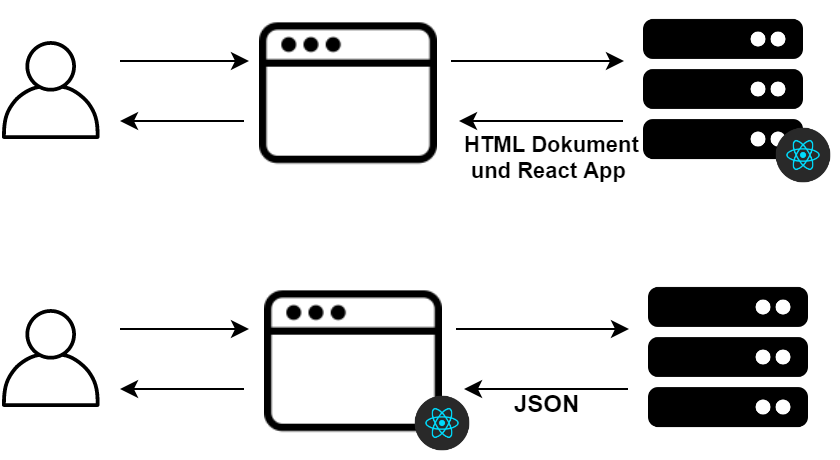
\includegraphics[width=12cm]{images/react}
  \caption{Universal Anwendung}
  \label{Universal Anwendung}
\end{figure}
\\
Beim Aufrufen einer Universal rendering Anwendung sendet der Browser
zuerst eine Anfrage an den Server. 
Dieser generiert aus einem Single Page Framework ein HTML Dokumemt,
in dem das Framework auf dem Server gerendert wird. 
Das HTML Dokument wird zusammen mit den benötigten Scripts eines clientseitiges Frameworks
an den Browser gesendet.
Ab diesem Zeitpunkt kann die Seite für den Anwender dargestellt werden, 
er erhält den First Contentful Paint (FCP). 
Anschließend lädt der Browser im Hintergrund eine Single Page Application herunter
und startet sie. 
Jetzt funktioniert die Anwendung wie eine Single Page Application und 
verwendet Client Side Rendering. Abbildung \ref{Universal Anwendung} zeigt wie bei dem 
ersten Aufrufen der Anwendung eine \textit{React} Anwendung auf dem Server verwendet wird,
zum generieren, rendern, eines HTML Dokuments. 
Nach dem darstellen des HTML Dokuments auf der Clientseite, 
wird die gleiche React Anwendung auf dem Client initalisiert.
\\
\\
Da die erste Antwort vom Server gerendert wird, enhtält sie Daten und ist
indexierbar. Dadurch ist die Suchmaschinenoptimierung von Universal Anwendungen einfacher
als rein clientseite Anwendungen, die beim ersten Aufrufen nur mit einem Template
HTML Dokument Antworten.
\begin{figure}[h]
  \centering
  
\includegraphics[width=10cm]{images/universalseo}
  \caption{Suchmaschinencrawler erhalten ein gerendertes HTML Dokument}
  \label{Suchmaschinencrawler erhalten ein gerendertes HTML Dokument}
\end{figure}
\\
Um dies zu ermöglichen kombiniert Universal Rendering mehrere Technologien. 
Es wird Isomorphic JavaScript verwendet um JavaScript auf dem Server und Client auszuführen, 
ein virtueller DOM für das Rendern auf dem Server und 
Code Hydration für den Wechsel zwischen server zu clientseitigen Rendern. \cite{tarkus_alabes}

\subsection{Isomorphic JavaScript}
\label{subsec:Isomorphic JavaScript}
Isomorphic Javascript oder auch Universal Javascript genannt, 
beschreibt JavaScript Code der auf der Server- und Clientseite ausführbar ist. 
Die JavaScript Laufzeitumgebung Node.js ermöglichen dabei 
das Ausführen von JavaScript-Code auf dem Server. 
Damit erlaubt Isomorphic JavaScript, 
in Kombination mit einem virtuellen DOM, moderne clientseitige Frameworks auf der Serverseite auszuführen. 
Dies verhindert auch das Problem der Code Duplikation, 
da es möglich ist den gleichen JavaScript Code auf dem Server und Client auszuführen, 
was die Wartbarkeit und Testbarkeit verbessert. \cite{airbnbeng_2013}

\subsection{Virtuelles DOM}
\label{subsec:Virtuelles DOM}
Das Virtuelle Document Object Model
oder auch virtuelles DOM (eng. virtual DOM) ermöglicht 
as Rendern moderner Web Anwendungen auf dem Server.
\\
\\
Bei modernen JavaScript Frameworks wie \textit{React}, 
VueJs und \textit{Angular} wird das HTML vollständig vom Framework kontrolliert. 
So kann das Framework einfach das HTML manipulieren und stellt sicher, 
dass der Zustand (engl. state) der Anwendung gleich mit dem Interface ist. 
So kann zum Beispiel bei einer Todo List Anwendung mit \textit{React} sichergestellt werden, 
dass beim Löschen einer Aufgabe der Zustand synchron mit dem Interface ist. 
Moderne JavaScript Frameworks garantieren, 
dass das Interface immer mit dem Zustand synchron ist und aktualisiert das Interface, 
sobald sich der Zustand ändert. 
Dabei wird ein virtuelles Document Object Model (virtual DOM) verwendet.
\\
\\
Das Document Object Model ist eine Datenstruktur in Form eines Baumes, 
die erzeugt wird, wenn der Browser das HTML Dokument rendert. 
Ein aktualisieren des Inhaltes einer Website ist nur möglich, 
durch Manipulation des DOMs, wofür Javascript eine API bietet. 
Beispielsweise kann über “document.createElement” ein HTML Element 
an den aktuellen DOM angehängt werden. 
Bei modernen Webanwendungen muss das DOM häufig aktualisiert werden. 
Da die DOM Bäume vieler Anwendungen sehr groß sind, 
verwenden viele Frameworks ein virtuelles DOM um die 
Aktualisierung zu beschleunigen. 
\\
\\
Das virtuelle DOM ist eine Abstraktion des HTML-DOM und 
von den Browser spezifischen Implementierungsdetails getrennt. 
Das virtuelle DOM ist eine lokale Kopie des HTML- DOMs, 
dargestellt in Form einer JavaScript Struktur. 
Dies erlaubt es Frameworks, 
Berechnungen abstrakt durchzuführen und Änderungen im DOM des Browsers 
zu überspringen die oft langsam und browserspezifisch sind.
\\
\\
Wenn sich der Zustand einer Anwendung ändert, 
sollten möglichst wenig Elemente im HTML-Dom manipuliert werden. 
Dafür gibt es zwei Ansätze bei aktuellen clientseitigen Frameworks:

\begin{itemize}
  \setlength\itemsep{1em}
  \item Bei \textit{React} wird die ganze Seite neu gerendert. 
  Wenn sich der Status der Anwendung ändert, 
  wird ein virtuelles DOM im Speicher generiert 
  und mit dem vorhandenen DOM verglichen. 
  Anschließend berechnet \textit{React} die Änderungen und führt diese 
  Änderungen im HTML- DOM durch. 
  Dieses Vorgehen ist performanter als direktes manipulieren 
  des Document Object Models.

  \item \textit{Angular} und Vue.js benutzen sogenannte Observer. 
  Dabei werden  Zustandsvariablen von Observern überwacht. 
  Sobald eine Änderung stattfindet, 
  werden nur die DOM-Elemente aktualisiert, 
  bei denen sich die Variablen geändert haben. 
  Um diesen Vorgang zu beschleunigen 
  wird auch hier ein virtuelles DOM verwendet, 
  um die Änderungen performanter durchzuführen. 
  Anschließend wird nur das sich ändernde Element im HTML- DOM aktualisiert.
\end{itemize}
Neben dem Verwenden auf der clientseite, 
ermöglichen virtuelle Document Object Models, 
erst das serverseitige rendern moderner Single Page Applications. 
Dadurch, dass das virtuelle DOM in Form von JavaScript dargestellt wird und 
somit unabhängig von dem Browser ist, 
ist es möglich, dies auf der Serverseite zu verwenden. 
Beim ersten Aufrufen einer Universal Rendering Webseite, 
wird das virtuelles DOM verwendet um ein HTML Dokument zu generieren. 
Der Client kann sofort nach dem Erhalten des Dokumentes mit dem rendern beginnen und 
es somit zeitnah für den Benutzer darstellen. \cite{krajka_2015}
\\
\\
Vue.js und \textit{React} besitzen für das Serverseitigen rendern eine \textit{renderToString()} Funktion. 
Diese Funktion erzeugt aus der aktuellen Instanz des Frameworks, 
auf der Serverseite, 
mithilfe eines virtuellen DOM ein HTML String. 
Dieser wird dem Client beim ersten Aufrufen der Website zurückgegeben.
\\
\\
Das rendern auf der Serverseite kostet allerdings Zeit und Performance. 
Das Rendern einer 1 Megabyte Anwendung mithilfe der \textit{renderToString() }
Funktion benötigt bis zu 1 Sekunde. 
Zusätzlich läuft die render Funktion in Node.js, 
was bedeutet, sie ist single-threaded und skaliert nicht gut. 
Dadurch erhöht sich die TTFB, je größer die Website wird. 
Ein Ansatz dies zu verhindern ist die Verwendung von renderToStream() anstatt renderToString. 
Dabei erzeugt der Server einen asynchronen HTML Stream an Daten, 
dies ermöglicht dem Browser die Seite zu rendern, 
bevor die Antwort abgeschlossen ist. 
Dadurch bleibt die TTFB gleich und 
wird nicht erhöht sich nicht durch größere Webseiten. 
Eine weitere Möglichkeit zur Verbesserung der TTFB und Entlastung des Servers, 
ist das Verwenden von Caching.

\subsection{Caching}
\label{subsec:Caching}
Mithilfe von Caching auf der Serverseite ist es möglich, 
die Zeit bis zum TTFB weiter zu verkürzen. 
Dies kann dann eingesetzt werden, 
wenn der Inhalt der aufgerufenen Seite dynamisch und nicht benutzerabhängig ist. 
Ist dies der Fall, kann durch Microcaching, 
eine Caching Technik die Inhalte nur für sehr kurze Zeiträume zwischenspeichert, 
die Ladezeiten und Auslastung des Servers vermindert werden. 
Da der Inhalt nur für einige Sekunden gecacht wird, 
bekommt der Benutzer keine veralteten Inhalte angezeigt. \cite{garett_2015}
\begin{figure}[h]
  \centering
  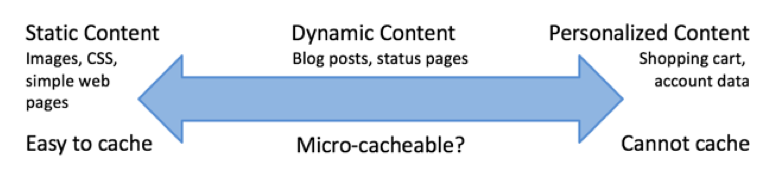
\includegraphics[width=10cm]{images/caching}
  \caption{Welche Daten können gecacht werden \cite{garett_2015}}
\end{figure}
\\
Durch das Caching verbessert sich die Server Performance, 
da nicht bei jedem erneuten Aufruf ein HTML Dokument mithilfe des virtuellen DOMs und 
der jeweiligen \textit{rendernToString()} Methode generieren werden muss. 
\\
\\
Bei modernen Web-Frameworks wie, Vue, 
lässt sich sogar direkt in dem JavaScript Code definieren, 
wie lang die jeweiligen Komponenten eines HTML Dokuments gecacht werden. 
\\
\\
Nachdem der Server mit dem statischen HTML Dokument dem Client geantwortet hat, 
beginnt die Client Side Hydration.

\subsection{Clientseitige Hydration}
\label{subsec:Clientseitige Hydration}
Client Side Hydration oder auch Rehydration genannt, 
bezieht sich auf den clientseitigen Prozess, 
in dem die Clientseite, 
den vom Server gesendeten statischen HTML-Code übernimmt und 
in ein dynamisches DOM verwandelt, 
das auf die clientseitige Datenänderungen und Benutzerinteraktionen reagiert. 
\\
\\
Beim ersten Laden einer Universal Website antwortet der Server mit einem, 
durch den virtuellen DOM, gerenderten HTML Dokument. 
Mithilfe dieses HTML erreicht man einen schnellen First Contentful Paint, 
allerdings ist die Seite ist noch nicht interaktiv. 
Da schon gerendertes HTML vorhanden ist, 
wird dies nicht weggeworfen. Stattdessen wird das HTML "hydrated", 
dadurch wird das statische HTML interaktiv. 
\\
\\
Dabei ist die Hydration auf der Client Side nur möglich, 
wenn das HTML des Servers identisch mit dem generierten HTML des jeweiligen 
Client-side Frameworks ist. 
Unterscheiden sich die jeweiligen Markup Dokumente, 
kommt es zu einem Fehler und der Hydration Vorgang schlägt fehl. 
Sind die Dokumente gleich findet die Hydration statt.
\\
\\
Hydration verbessert die Zeit bis zum FCP, 
aber es entsteht ein negativer Einfluss auf die Zeit bis die Website interaktiv ist. 
So wirkt die Seite nach dem FCP für den Anwender interaktiv, 
obwohl sie zu diesem Zeitpunkt noch statisch ist. 
Diese Zeit zwischen dem FCP und der TTI wird Uncanny Valley genannt. 
Je nach Anwendungsart ist das Uncanny Valley unterschiedlich problematisch. 
Bei einem Blog stellt dies kein Problem dar, 
da der User schon nach dem FCP die Artikel lesen kann. 
Schwieriger ist es bei einer Chat-App, 
hier kann der User erst antworten, 
nachdem die Hydration abgeschlossen ist. \cite{vue.jsserver-sideguide} \cite{arunoda}
\\
\\
\textbf{Lazy Hydration}
\\
Lazy Hydration ist eine Möglichkeit die Zeit bis eine Webseite Interaktiv ist, 
zu verbessern. Dabei wird die Hydratation des vorgerenderten HTML Dokuments des Servers verzögert und 
inkrementell hydriert. Mit Lazy Hydration ist möglich, 
bei Website zu implementieren, 
dass die Kommentare am Ende der Website erst hydriert werden, 
wenn sie für den Nutzer sichtbar sind. 
Dies beschleunigt das Hydrieren der wichtigen Elemente für den Anwender und sorgt damit dafür, 
dass die Website schneller interaktiv wird und sich die TTI verbessert. 
Des weiteren ist es auch möglich, 
statische Komponenten wie den Artikel Inhalt, nicht zu hydrieren.
\begin{figure}[h]
  \centering
  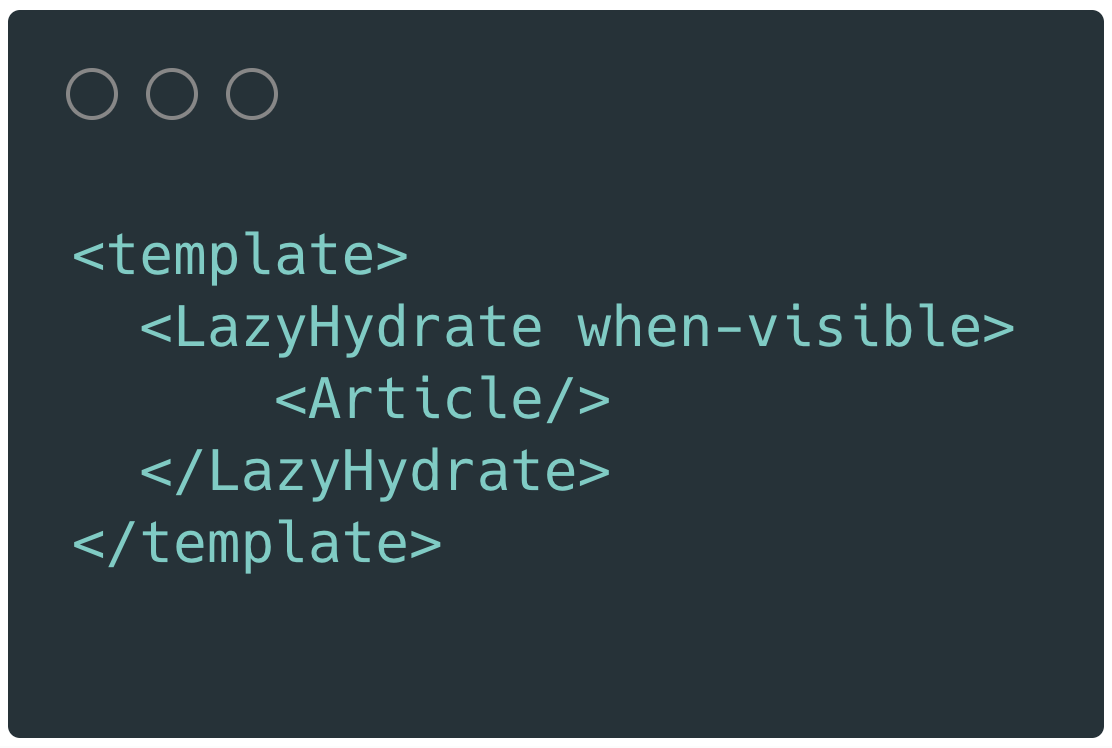
\includegraphics[width=5cm]{images/LazyHydration}
  \caption{Lazy Hydratation mit \textit{vue-lazy-hydration}}
  \label{Lazy Hydratation mit vue-lazy-hydration}
\end{figure}
\\
Vue.js bietet mit der Bibliothek \textit{vue-lazy-hydration }
eine einfache Möglichkeit um Lazy Hydration zu implementieren. 
Die Abbildung \ref{Lazy Hydratation mit vue-lazy-hydration} zeigt wie der Artikel erst Hydriert werden kann, 
wenn er für den Nutzer sichtbar wird. \cite{maoberlehner_2018}
\subsection{Rendering Ablauf}
\label{subsec:Rendering Ablauf}
Die Architektur einer Universal Anwendung, ähnelt der einer clientseitigen Anwendung. Eine
zweite Präsentationsschicht \ref{Universal Rendering Architektur} ist auf der Serverseite zum generieren des HTMLS Dokumentes beim
ersten Aufrufen der Webseite nötig.
\begin{figure}[h]
  \centering
  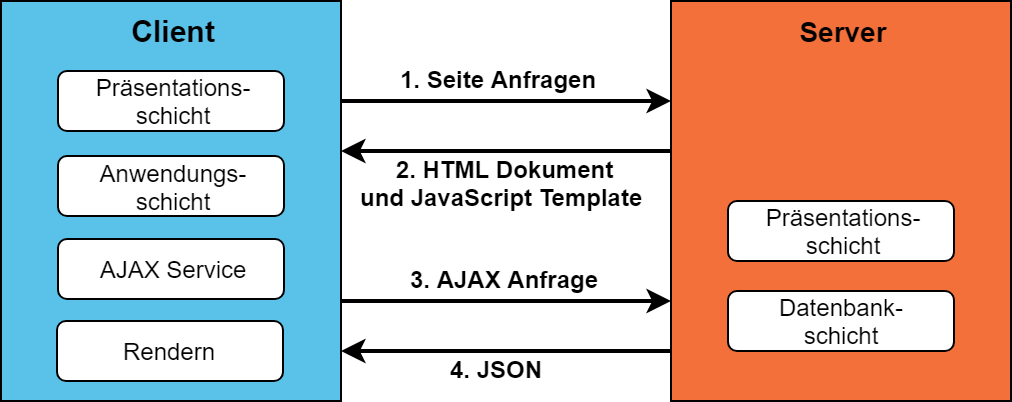
\includegraphics[width=12cm]{images/universal}
  \caption{Universal Rendering Architektur}
  \label{Universal Rendering Architektur}
\end{figure}
\\
Folgende Schritte werden beim Aufrufen einer Universal Anwendung aufsgeführt:
\begin{enumerate}
  \setlength\itemsep{1em}
  \item Beim ersten Aufrufen einer Seite, sendet der Client eine Anfrage an den Server.
  \item Auf der Serverseite läuft ein Node.js Prozess, 
  dieser generiert mithilfe eines virtuellen DOMs 
  ein statisches HTML Dokument als Antwort auf die Anfrage. 
  Das HTML ist auf den Anwender angepasst und enthält bereits anwenderspezifische Informationen.
  \item Der Server sendet das vorgerenderte Dokument an den Client.
  \item Der Client erhält das Dokument und rendert es. 
  Zu diesem Zeitpunkt sieht der Anwender die Webseite, 
  kann aber noch nicht mit ihr interagieren.
  \item Nachdem Erhalt des HTML beginnt die Client Side Hydration. 
  Der Client lädt dafür zunächst die benötigten Skriptdateien runter.
  \item Besitzt der Client die benötigten JavaScript Dateien, 
  wird die clientseitige Anwendung initialisiert. 
  Anschließend findet die Hydration statt und 
  das statische vorgerenderte HTML wird 
  durch ein dynamisches HTML von der clientseitigen Anwendung ersetzt und 
  anschließend zum DOM gerendert. 
  Ab diesem Zeitpunkt ist die Website für den Anwender interaktiv.
  \item Ab diesem Zeitpunkt werden alle Interaktionen und 
  Navigationen zwischen den Seiten durch Ajax Anfragen durchgeführt.
\end{enumerate}
\newpage
\subsection{Vorteile}
\label{subsec:Vorteile}
\begin{figure}[h]
  \centering
  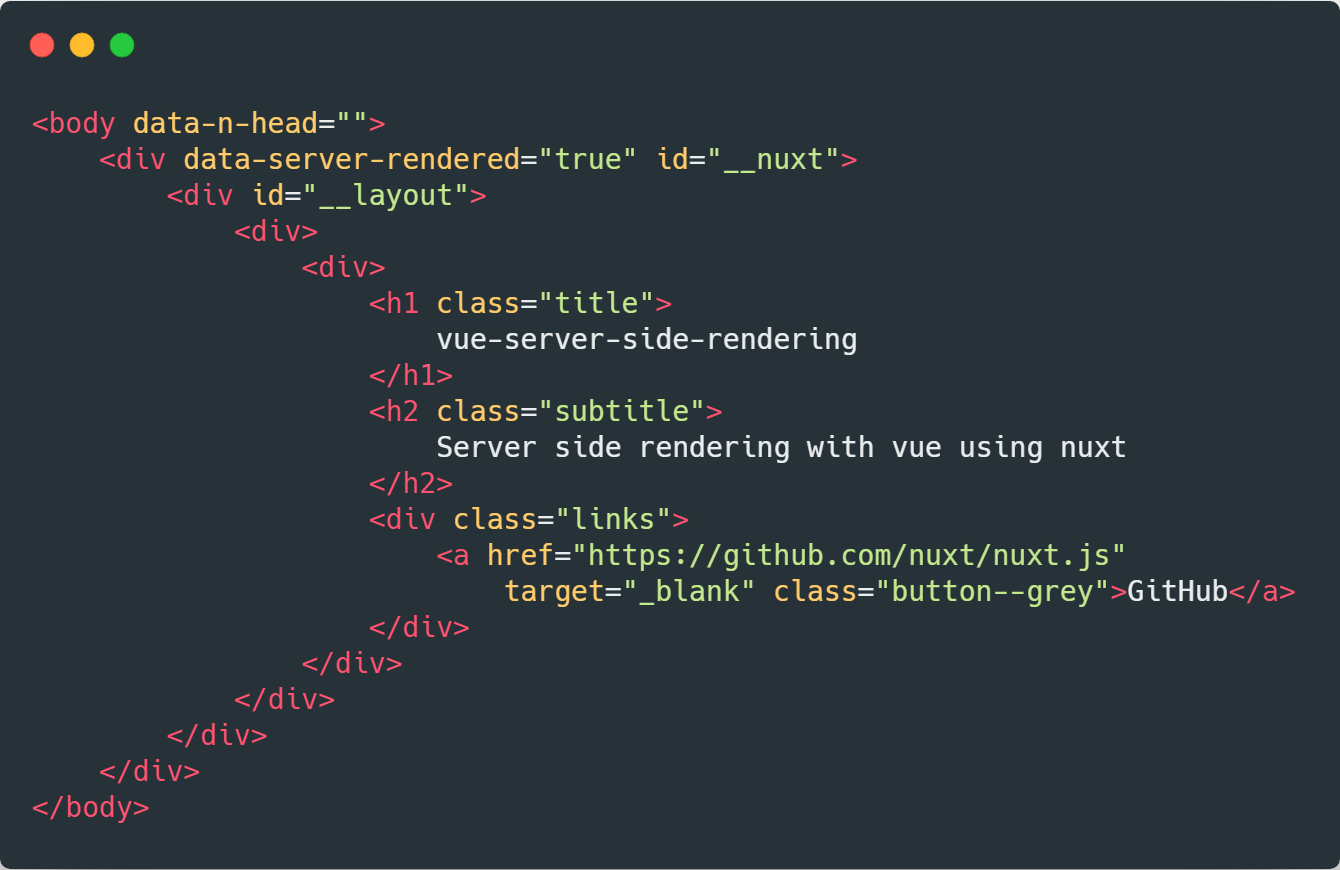
\includegraphics[width=12cm]{images/nuxt-body-first}
  \caption{HTMl Dokument einer Universal Anwendung}
  \label{HTMl Dokument einer Universal Anwendung}
\end{figure}
\begin{itemize}
  \setlength\itemsep{1em}
  \item Da beim ersten Aufrufen einer Universal Anwendung der Server mit einem HTML Dokument antwortet, 
  ist dieser Rendering Ansatz genauso SEO freundlich wie normale klassische serverseitige Webseiten. 
  Der Suchmaschinencrawler erhält ein indexierbares Dokument und muss nicht wie bei klassischen SPAs, 
  JavaScript Bundles laden und starten. 
  Abbildung \ref{HTMl Dokument einer Universal Anwendung}
  zeig den Body einer HTML Universal Anwendung, der im gegensatz zu Single Page Anwendungen Nutzer Daten
  enthält, da die erste Anfrage vom Server gerendert wurde.
  Des weiteren benötigt man bei Universal Rendering keine Hash am ende von URLs, 
  wodurch der Crawler zwischen verschieden Links auf der Seite unterscheiden kann. 
  Dies verbessert nicht nur die Indexierbarkeit, 
  sondern auch die Social Media Performance der Website. 
  Schreibt man einen Twitter Post mit einem Link zu einer Universal Anwendung, 
  so kann der Twitter Bot die Webseite einfach crawlen und eine Vorschau zu der Webseite generieren, 
  dass unter dem Tweet eingeblendet wird. 
  Bei einer SPAs ist dies nicht der Fall.
  \item Durch das Server Side Rendern der ersten Anfrage, 
  erhält der User eine schnelle Antwort auf die Anfrage und 
  muss nicht wie bei Single Page Anwendungen warten bis der Client alle Skripts geladen und 
  installiert hat. Die Zeit bis die Anwendung interaktiv ist, 
  ist größer als bei reinen serverseitigen Anwendungen, 
  aber mithilfe von lazy Hydration besser als bei SPAs. 
  \item Nach der Hydratation bei Universal Anwendungen, 
  läuft auf der Client Seite eine normale Single Page Applications. 
  Dies erlaubt wie bei SPAs eine Webseite anzubieten, 
  die benutzerfreundlich und interaktiv ist.
  \item Moderne Universal Rendering Frameworks sind komfortabel zu entwickeln. 
  So ist es möglich Programmcode einmalig zu schreiben und 
  die Frameworks rendern diesen server- und clientseitig. 
  So können komfortable SPA Frameworks zum entwickeln der Clientseite verwendet werden. 
  Dies macht die Anwendung einfacher zu Warten. 
  Das Verwenden von JavaScript auf dem Client und 
  Server vereinfacht zusätzlich das Entwickeln der Anwendung.
\end{itemize}

\subsection{Nachteile}
\label{subsec:Nachteile}
Das Verwenden von Universal Rendering löst viele Probleme, 
bringt aber auch neue Herausforderungen und 
Nachteile gegenüber klassischen Verfahren.
\\
\\
Der größte Nachteil von Universal Rendering ist, 
dass im Gegensatz zu clientseitigen Anwendungen, 
ein render Prozess auf dem Server laufen muss. 
Die Dynamik des serverseitigen Vorrenderns 
kann zu erheblichen Rechenaufwand auf dem Server führen, 
was wiederum Kosten verursacht. 
Dadurch, dass auf dem Server eine Node.js Instanz laufen muss, 
skaliert der Prozess nicht gut, 
da die Render- Funktionen synchron und singlethread sind. 
Dies erschwert die Skalierbarkeit und erhöht gleichzeitig noch die TTFB, 
da auf eine Antwort des Servers gewartet werden muss, 
da während dem Rendern des HTML Dokuments der Event Loop blockiert ist. 
Der Rechenaufwand kann zwar verkleinert werden, 
durch Caching und Memory Management, 
dies führt aber schnell dazu, 
dass die Anwendung komplex und unübersichtlich wird. 
Single Page Anwendungen haben dieses Problem nicht, 
da es ausreicht die Dateien statisch zu hosten, 
ohne einen serverseitigen Prozess. 
So skaliert eine SPA deutlich besser, 
da die Webseite vollständig auf der Clientseite gerendert wird.  
Bei einer erhöhten Benutzerzahl, 
ist die skalierung damit deutlich einfacher, 
da nur ein werden. 
Rein serverseitige Anwendungen benötigen zwar auch ein serverseitigen Prozess, 
lassen sich aber besser skalieren, 
da die Anfragen meist asynchron bearbeitet werden können. 
Dies führt zu einer besseren TTFB als bei Universal Rendering.
\begin{figure}[h]
  \centering
  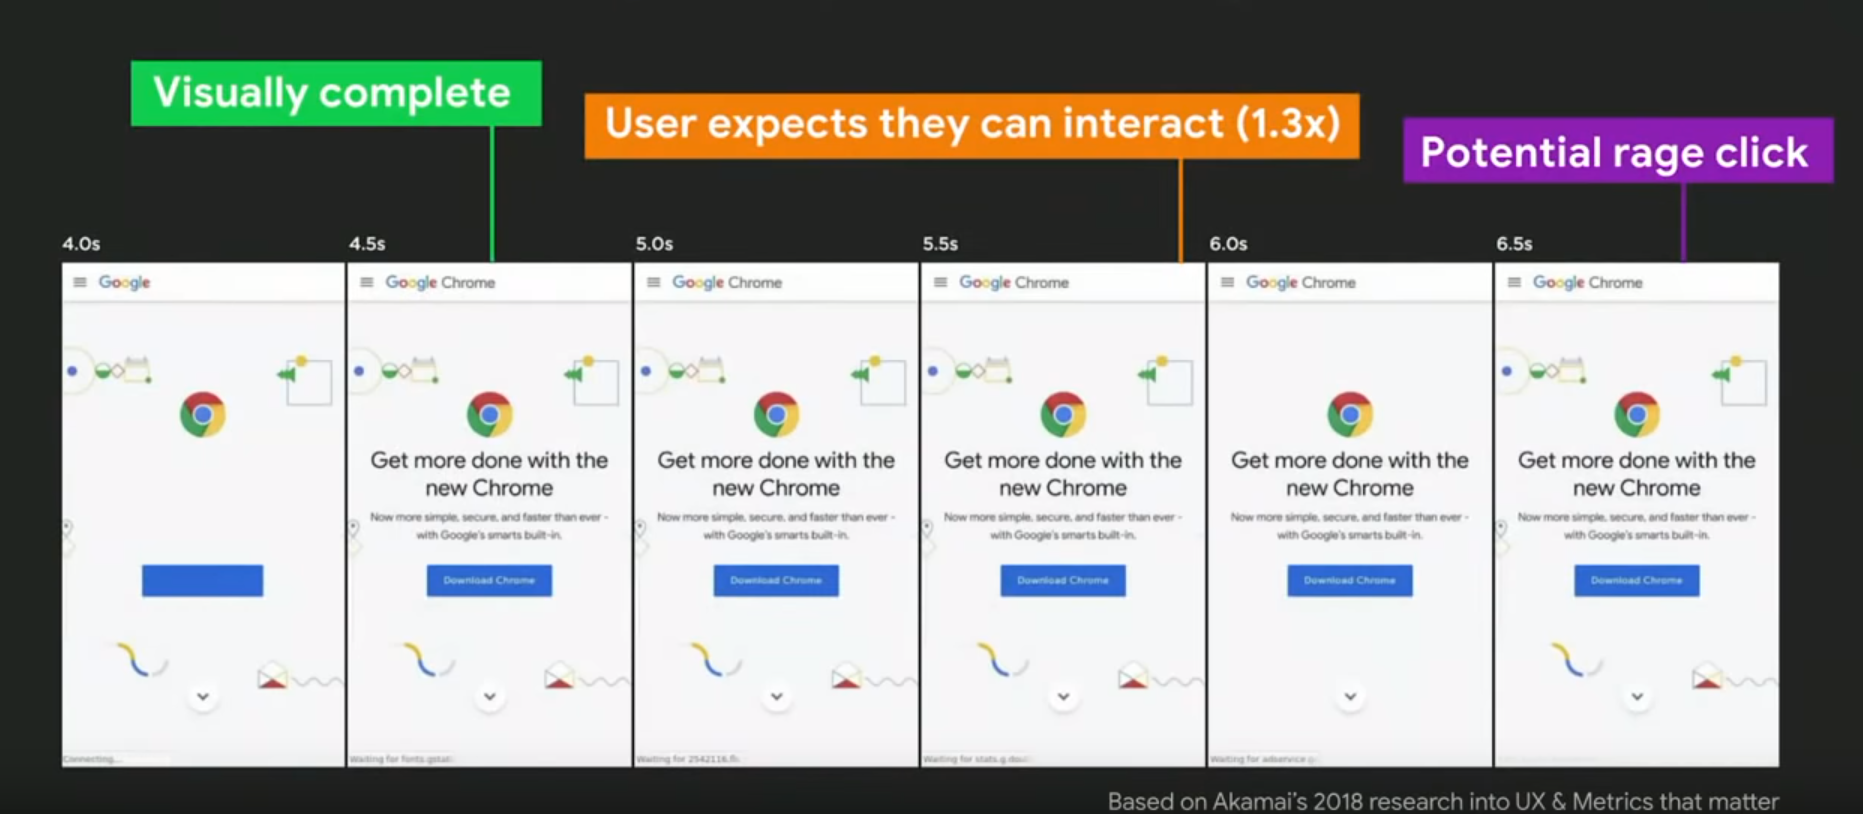
\includegraphics[width=10cm]{images/TimeToInteractive}
  \caption{Verspätete TTI \cite{osmani_2019}}
  \label{Verspätete TTI}
\end{figure}
\\
Ein weiteres Problem stellt die Time to Interactive (TTI) dar. 
Bei Universal Rendering erlaubt das Vorrendern auf dem Server, 
eine Website schnell darzustellen. 
Zu diesem Zeitpunkt kann der Anwender noch nicht mit der Seite interagieren. 
Wenn der Benutzer sehr schnell ist und auf eine Schaltfläche klickt, 
wird die Aktion erst ausgeführt wenn die clientseitige Hydration abgeschlossen ist. 
Je nach Art der Webseite kann dies zu Problemen führen wie Abbildung \ref{Verspätete TTI} zeigt


\subsection{Alternativen}
\label{subsec:Alternativen}
Eine Alternative zum Universal Rendering ist das clientseitige rendern mit Prerendering. 
Prerendering benötigt keinen vollständigen Server auf der Serverseite. 
Beim Prerendering werden vordefinierte Seiten der Anwendung im Vorraus als HTML kompiliert und 
statisch auf einem statischen Server gespeichert. 
\\
\\
Dies erlaubt es, beim Aufrufen mithilfe von Hydration, 
eine schnellere TTFB im Vergleich zu Universal rendering. 
Desweiteren ist auch keine Node.js Prozess auf dem Server nötig. 
Da die erste Antwort aber statisch und nicht dynamisch ist, 
erhält man beim ersten Aufrufen noch keine benutzerspezifischen Informationen. 
Wenn die Anwendung benutzerspezifische Daten enthält, 
wird in der Regel ein Skelett der Anwendung eingeblendet, 
bis die Clientside initialisiert ist und die Daten zur verfügung stehen. 
Durch die statisch generierten Seiten, 
ist die Anwendung einfacher zu Crawlen wie SPAs. 
Prerendering wird von Frameworks wie \textit{Peact}, 
Gatsby und Vuepress verwendet.
\begin{figure}[h]
  \centering
  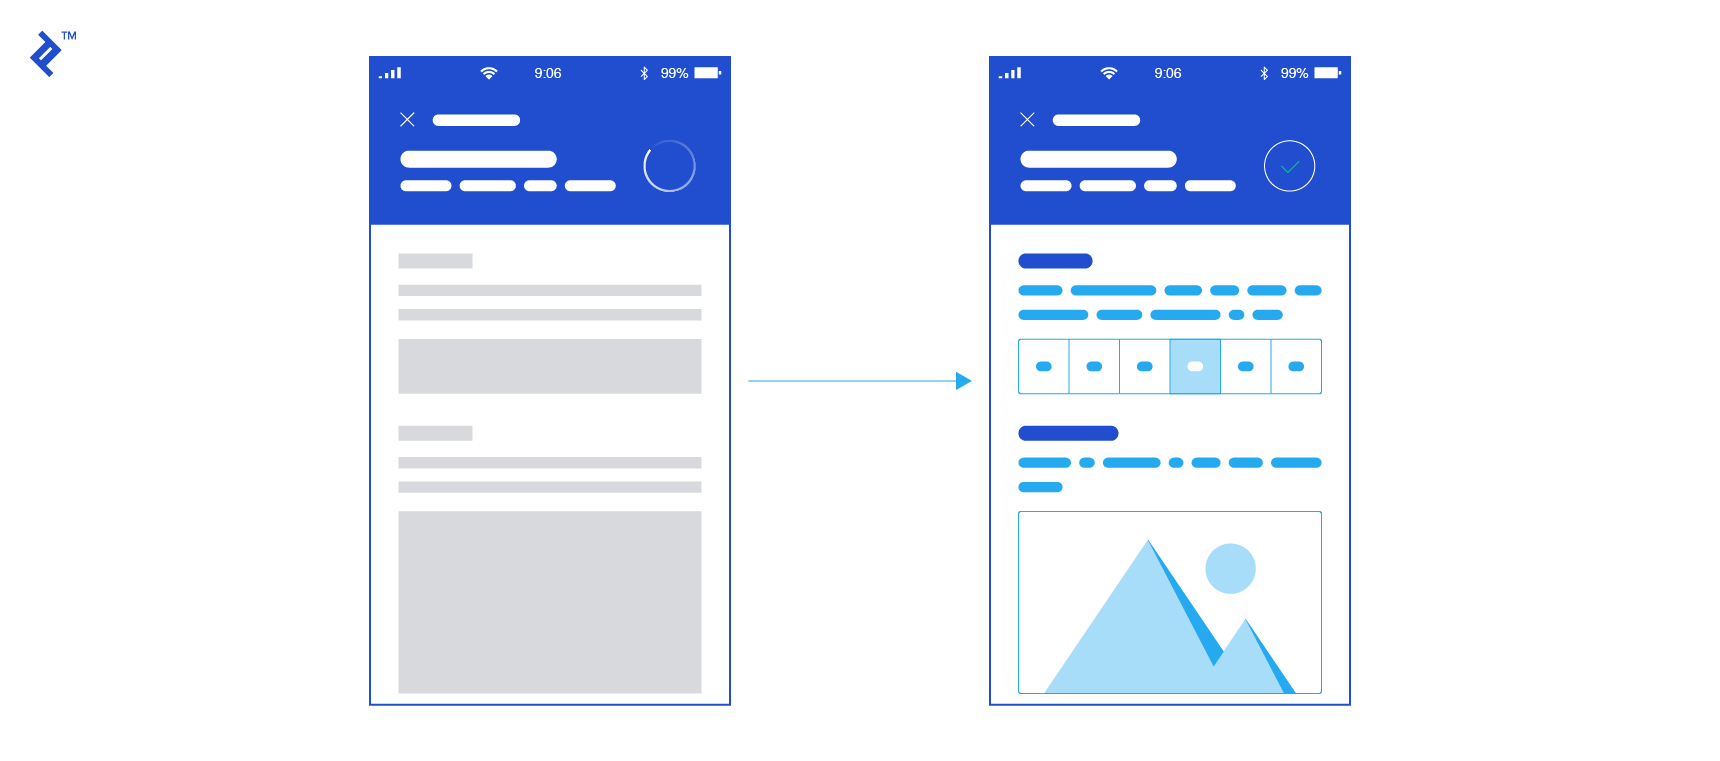
\includegraphics[width=9cm]{images/WebsiteSceleton}
  \caption{Skelett einer Webanwendung \cite{breux_2018}}
\end{figure}
\\
Wenn man nur die SEO einer Single Page Applications verbessern will, 
ist es auch möglich, 
wichtige Teile der Anwendung, 
wie die Kontakt oder About Seite, 
als statisches HTML ähnlich wie bei Prerendering zu speichern. 
So können diese Seiten einfach von einem Crawler indexiert werden.
\\
\\
Eine weitere Alternative ist das Verwenden von SPA in Kombination mit Headless Browsern zum vorrendern einer Webseite. 
Ein Headless Browser ist ein Browser, 
der meist auf den gängigen Rendering-Engines wie Chrome basiert, 
um Web-Inhalte darzustellen. Dieser ist aber “Kopflos”, was bedeutet, 
er besitzt keine UI Elemente. 
Ursprünglich wurden Headless Browser zum automatischen Testen von Webseiten entwickelt, 
sie können aber auch verwendet werden um Single Page Application auf dem Server zu rendern. 
\\
\\
Ruft ein Anwender oder ein Suchmaschinen Crawler eine Website auf, 
wird ein Headless Browser auf einem Server zum vorrendern verwendet. 
Dies verbessert wie bei Universal Rendering die Zeit bis zum FCP. Gleichzeitig verbessert sich die SEO, da der Crawler ein indexierbares HTML Dokument erhält. 
Problem dieses Vorgehens ist die Skalierbarkeit, 
da für jeden Nutzer ein neuer Headless Browser gestartet werden muss. 
Des weiteren muss die Webseite zweimal entwickelt werden, 
einmal für die SPA auf dem Client und ein zweites Mal für den Headless Browser. 
Dies ist komplex und fehleranfällig. Das hat zur Folge, 
dass in der Praxis diese Variante des Renderns nur sehr selten verwendet wird. 
Allerdings gibt es Dienstleister, wie Brome Bone, 
die verwendet werden können um dies zu vereinfachen, 
was aber zu weiteren Kosten führen kann.

\newpage
% -------------------------------------------------------------------------------------------------

\section{Frameworks}
\label{sec:Evaluation}
Universal Rendering Frameworks vereinfachen das Verwenden von clientseitigen Frameworks wie Vue, 
\textit{React} und \textit{Angular} zum Entwickeln für Universal Rendering Anwendungen. 

\subsection{React und Next.js}
\label{subsec:React und Next.js}
\textit{React} ist ein clientseitiges JavaScript Framework zum Erstellen von Benutzeroberflächen. 
Es wurde 2013 von Facebook veröffentlicht und ist aktuell eines der populärsten User Interface Frameworks. 
Da React ein virtuellen DOM besitzt, 
kann es serverseitig gerendert werden und eignet sich für Universal Anwendungen.
\\
\\
Da das Entwickeln von Universal Anwendungen schnell komplex wird und 
viele Aspekte beim Entwickeln beachtet werden müssen, 
hat \textit{ZEIT} das Open Source Framework \textit{Next.js}, 
basierend auf \textit{React} veröffentlicht. 
Dies vereinfacht das Erstellen von Universal Anwendungen mit \textit{React}.
\begin{figure}
  \centering
  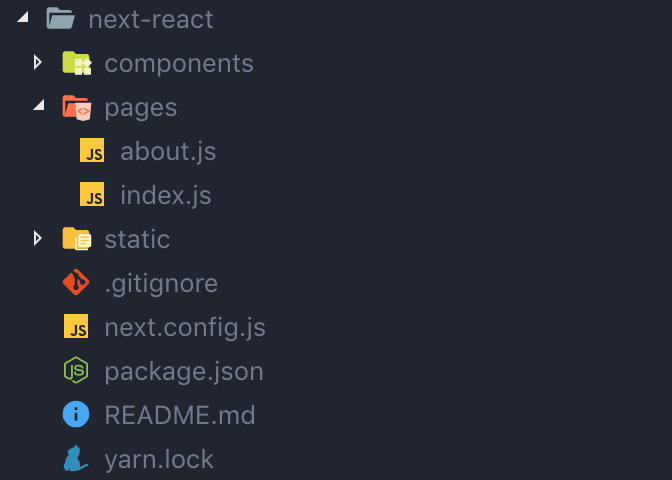
\includegraphics[width=5cm]{images/nextprojectStructure}
  \caption{\textit{Next.js} Projektstruktur\cite{arunoda}}
  \label{Next.js Projektstruktur}
\end{figure}
\\
\textit{Next.js} automatisiert das serverseitige Rendern, 
so kann die Anwendung wie eine normale \textit{React} SPA entwickelt werden und 
\textit{Next.js} automatisiert das Vorrendern der Website. 
Gleichzeitig hilft \textit{Next.js} mit der Wartbarkeit der Webseite, 
indem es einen Dateibasierten Ansatz zum Verwalten der Seiten, 
Komponenten und Routen verwendet. 
Wird beispielsweise eine about.js Datei unter dem Pfad /pages/about.js erstellt, 
kann die Seite einfach über die URL /about aufgerufen werden\ref{Next.js Projektstruktur}. 
\textit{Next.js} stellt dabei sicher, 
dass die Seite automatisch auf dem Server vorgerendert wird und 
anschließend als SPA auf dem Client verfügbar ist. 
\begin{figure}
  \centering
  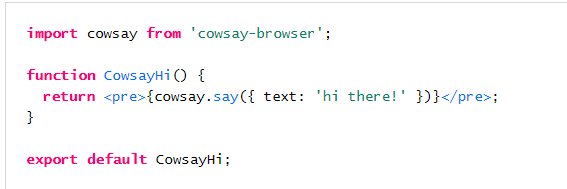
\includegraphics[width=10cm]{images/CodeSplitting}
  \caption{CodeSplitting in \textit{Next.js} \cite{arunoda}}
  \label{CodeSplitting in Next.js}
\end{figure}
\\
Neben Universal Rendering, bietet \textit{Next.js} automatisches “Code Splitting”. 
Bei klassischen Single Page Anwendungen wird der gesamte JavaScript Code 
zu Beginn der Anwendung geladen. 
Dies erhöht die Zeit bis zum FCP, da der User warten muss, 
bis die gesamte Seite vom Client geladen ist. 
Besonders bei mobilen Internet ist dies langsam. 
Dieser Ansatz kann zu unnötigen Ladezeiten führen, 
da möglicherweise auch JavaScript von Teilen der Anwendung geladen wird, 
die der Benutzer gar nicht aufrufen will. 
Code Splitting kann eingesetzt werden um dies zu verhindern. 
Dabei wird der Code aufgeteilt und nur der Teil geladen, 
den der Benutzer im Augenblick aufruft. 
Dies verringert die Zeit bis zum FCP und ist vorteilhaft für Mobilnutzer, 
da die Ladezeiten minimiert werden.
\textit{Next.js} teilt den Code automatisch anhand von Seitengrenzen auf. 
Nur beim in Aufrufen der in Abbildung \ref{CodeSplitting in Next.js} gezeigten Seite,
wird der Code von dem cowsay-browser geladen.
Ruft der Benutzer beispielsweise die Route /about auf, 
lädt der Client nur den JavaScript Code für diese Seite der Anwendung herunter.
\begin{figure}
  \centering
  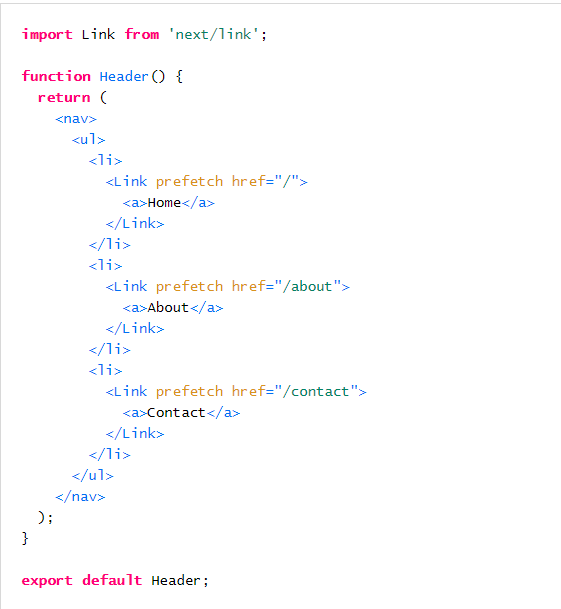
\includegraphics[width=10cm]{images/prefetchnext}
  \caption{Prefetching in \textit{Next.js}}
  \label{Prefetching in Next.js}
\end{figure}
\\
\textit{Next.js} bietet zudem eine Möglichkeit zum Prefetching, 
dem Vorausladen von Seiten. 
Das Vorausladen von Seiten kann in Kombination mit serverseitigen rendern verwendet werden, 
um ohne Ladezeit zwischen verschieden Seiten der Anwendung zu navigieren. 
\textit{Next.js} verwendet ein Link HTML Tag zum Navigieren zwischen Seiten, 
dieses bietet die Funktion eines “prefetch” Attributes. 
Ist das Attribute gesetzt, 
lädt JavaScript die verlinkte Route im Hintergrund herunter. 
Klickt der Benutzer den Link, 
wird sofort navigiert und die Seite dargestellt. 
Abbildung \ref{Prefetching in Next.js} zeigt eine Anwendung mit 3 Routen für /, /about und /contact. 
Da bei jedem Link Tag das prefetch Attribut vorhanden ist, 
wird \textit{Next.js} die Seiten im Hintergrund herunterladen. 
So wird dem Benutzer sofort nach klicken des Links die About Seite angezeigt.
\\
\\
Zudem unterstützt \textit{Next.js} das dynamische Importieren von JavaScript Modulen sowie Komponenten. 
Dies erlaubt das Importieren von Komponenten zur Laufzeit. 
Mit dem dynamischen Laden von Komponenten ist es möglich, 
nur die für den Nutzer sinnvollen Teile der Seite zu laden. 
Beispielsweise kann je nachdem, 
ob die Webseite von einem Mobilgerät oder eines Desktops aufgerufen wird, 
unterschiedliche Komponenten dynamisch geladen werden. 
\\
\\
Für das Veröffentlichen einer \textit{Next.js} Webseite, 
muss zuerst die Anwendung über npm run build gebaut werden. 
Dies fügt die nötigen Polyfills ein, 
damit die Webseite auch auf älteren Browsern läuft und 
verkleinert (minify) die Skripte für eine bessere Performance. 
Anschließend kann der Node.js Server Prozess über npm run start gestartet werden. 
Die Universal Rendering Seite kann jetzt über einen spezifizierten Port aufgerufen werden. \cite{arunoda} \cite{AlexMoldovan-siderenderinginReact}
\subsection{Vue.js und Nuxt.js}
\label{subsec:Vue.js und Nuxt.js}
Vue ist ein weiteres clientseitiges JavaScript Framework 
zum Erstellen von Single Page Application. 
Es wurde 2014 von Evan You veröffentlicht und 
wird seitdem von der Community weiterentwickelt. 
In den letzten Monaten ist die Popularität von Vue gestiegen und 
es ist aktuell das Projekt mit den meisten Sternen auf Github. 
Vue.js besitzt auch ein virtuelles DOM, 
was Universal rendern ermöglicht. 
Um dies zu vereinfachen gibt es das Open Source Framework \textit{Nuxt.js}. \cite{vue.jsserver-sideguide}
\\
\\
\textit{Nuxt.js} ähnelt stark \textit{Next.js}, 
der einzige Unterschied ist, 
dass es Vue.js anstelle von \textit{React} für das Schreiben des Interface Codes verwendet. 
\textit{Nuxt.js} hat den gleichen dateibasierten Ansatz und ermöglicht automatisches Universal rendern von Anwendungen.
\\
\\
Neben dem Universal Rendering bietet \textit{Nuxt.js} auch die Möglichkeit statische Dateien aus der Anwendung zu generieren und 
prerendering zu verwenden.
Über npm run generate generiert \textit{Nuxt.js} ein dist Ordner mit einer index.html Datei 
die einfach von einem Server bereitgestellt werden kann. 
So kann die Seite als klassische SPA mit vorgerenderten Seiten für eine bessere Suchmaschinenoptimierung verwendet werden.

\subsection{Angular Universal}
\label{subsec:Angular Universal}
\textit{Angular}.js (\textit{Angular} 1) ist ein weiteres Clientseitiges Framework, 
dass 2010 von Google veröffentlicht wurde. 
Mit der Einführung von \textit{Angular} 2 wurde es durch den virtuellen DOM möglich, 
das \textit{Angular} Framework auch als Universal Anwendung zu benutzen, 
genannt \textit{Angular} Universal. 
\\
\\
Ab \textit{Angular}-Version 4, 
ist die Universal Funktion nativ im Framework als Modul eingebunden. 
Über das \textit{@angular/platform-server} Modul ist es mit wenigen Schritten möglich, 
eine Universal Anwendung zu entwickeln. 
Das Modul enthält ähnlich wie \textit{React} eine Methode, 
welche die Anwendung rendert und das Resultat als String zurückgibt. 
Dies ermöglicht das Vorrendern der Anwendung auf dem Server. 
Auf der Clientseite findet anschließend die Hydration statt und 
die Anwendung wird interaktiv. 
\\
\\
Im Gegensatz zu \textit{Nuxt.js} und \textit{Next.js} bietet \textit{Angular} Universal keine 
“out of the Box” Universal Rendering Möglichkeit, 
es müssen die benötigten Module importiert werden um dies zu erreichen. 
\\
\\
\textit{Angular} bietet das Hilfswerkzeug \textit{Angular} CLI (Command Line Interface) an, 
dass beim Erstellen einer Universal Anwendung hilft. 
Die \textit{Angular} CLI ermöglicht das Erstellen und Ausführen einer \textit{Angular} Anwendung und 
erlaubt es prerendering oder Universal Rendering zu verwenden. 

\newpage
% -------------------------------------------------------------------------------------------------

\section{Universal Rendering in der Praxis}
\label{sec:Universal Rendering in der Praxis}

Die Zeit bis eine Webseite geladen ist und der Benutzer Inhalte sehen kann, 
wird immer wichtiger. 
Laut einem Radware-Bericht war der durchschnittliche Benutzer 1999 bereit, 
8 Sekunden auf das Laden einer Seite zu warten. 
Bis 2010 gaben 57\% der Online-Käufer an, dass sie eine Seite nach 3 Sekunden laden verlassen würden. 
Amazon und Walmart bestätigen, dass für alle 100 Millisekunden Verbesserungen der Ladezeit, 
der Umsatz der Website bis zu 1\% steigt. \cite{young} \cite{einav_2019}
\\
\\
Gerade bei Online Shops ist das Verwenden von Universal rendering sinnvoll, 
da der Benutzer schnell die Verkaufsartikel angezeigt bekommt und nicht warten muss, 
bis die ganze Seite initialisiert ist. 
Des weiteren können die Artikel einfach von Suchmaschinen indexiert werden, 
wodurch sie besser von Benutzern gefunden werden können.
\begin{figure}
  \centering
  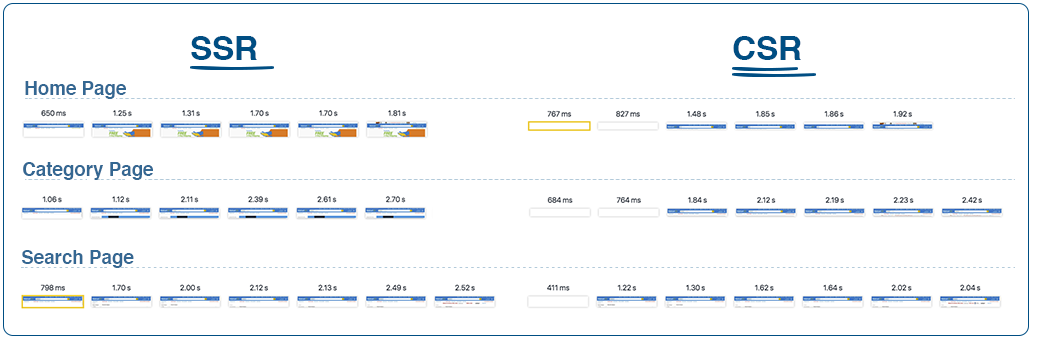
\includegraphics[width=12cm]{images/ssrvscsrwallmart}
  \caption{Verbesserung des First Contentful Paint der Walmart Webseite}
  \label{Verbesserung des First Contentful Paint der Walmart Webseite}
\end{figure}
\\
Wegen der besseren Performance für den Nutzer und bessere SEO, 
hat sich Walmart 2016 entschieden, 
Universal rendering einzusetzen. 
Walmart hat dafür ein eigenes Framework namens Electrode-io veröffentlicht, 
was es erlaubt \textit{React} Universal Anwendungen für eine große Zahl an Nutzer zu entwickeln. 
Walmart hat Electrode-io Erweiterungen veröffentlicht, 
die mittels Caching und überspringen des serverseitigen Vorrendern von Teilen der Webseite, 
die für den Anwender nicht Sichtbar sind, 
die \textit{renderToString()} Methode von \textit{React} beschleunigt. 
Abbildung \ref{Verbesserung des First Contentful Paint der Walmart Webseite} zeigt auf der linken Seite, 
wie durch das serverseitige Vorrendern, 
die Webseite schneller lädt. Beim clientseitigen Rendern hingegen, 
muss der Benutzer 1 Sekunde warten bis die Seite geladen ist. 
Bei schlechtem Internet, vergrößert sich diese Ladezeit schnell.
\\
\\
Airbnb ist für eine bessere Ladezeit ihrer Webseite 
von dem serverseitigen Framework Ruby on Rails zu Universal Rendering mit \textit{React} und Node.js gewechselt. 
\newpage
% -------------------------------------------------------------------------------------------------

\section{Fazit}
\label{sec:Fazit}

\subsection{Wann ist Universal Rendering sinnvoll}
\label{subsec:Wann ist Universal Rendering sinnvoll}
Das Verwenden von Universal Rendering bringt viele Vorteile und 
löst das Performance und SEO Problem von Single Page Applications. 
Universal Anwendungen bringen Kosten durch Server Performance und sind aufwendig zu skalieren. 
Aus diesen Gründen ist das Verwenden von Universal Rendering nicht immer sinnvoll und notwendig.
\\
\\
Für Web Anwendungen bei denen sich der Benutzer anmelden muss, 
um eine für den Nutzer privaten Teil der Webseite aufzurufen, 
reicht eine Single Page Anwendung aus. 
Beispielsweise Googles Gmail Webanwendung ist eine SPA, 
da eine Anmeldung notwendig ist um die Emails abzurufen. 
Suchmaschinen Crawler haben keinen Zugriff auf die Email-Anwendung und 
können diese nicht indexieren. 
Da die Anmeldeseite statisch ist, 
kann hier prerendering verwendet werden um diese für die Crawler indexierbar zu machen. 
Universal rendering wäre hier nicht vorteilhaft.
\\
\\
Anwendungen die performant sein sollen, 
aber nicht dynamisch, können mit serverseitigen Rendern und 
Ajax erreicht werden. Beispielsweise die Nachrichten Plattform Hacker News, 
die primär Links zu Artikeln anzeigt, 
verwendet serverseitiges rendern ohne Client Side Framework. 
Dies führt zu einer guten Indexierbarkeit von Suchmaschinen und 
einer schnellen Time to interaction. Beim Aufrufen der Webseite, 
bekommt der Benutzer schnell die Links angezeigt und 
kann mit ihnen interagieren. 
\begin{figure}
  \centering
  
\includegraphics[width=10cm]{images/HackerNews}
  \caption{Die Webseite HackerNews}
  \label{Die WEbseite HackerNews}
\end{figure}
\\
Das Einsetzen einer Universal rendering Anwendung ist bei folgenden Punkten sinnvoll: 
\begin{itemize}
  \setlength\itemsep{1em}
  \item Die Webseite soll durch Suchmaschinen indexiert werden können. 
    Neue Nutzer sollen die Seite durch Suchmaschinen finden.
  \item Die Inhalte der Webseite sollen auf sozialen Medien geteilt werden können. 
  \item Die Ladezeit der Webseite ist für den Benutzer wichtig, 
  da es sonst zu einer hohen Absprungrate kommt.
  \item Es gibt ausreichend Ressourcen zum Mieten von Servern, 
  insbesondere wenn die Webseite von vielen Nutzern genutzt wird. 
\end{itemize}
\subsection{Ausblick}
\label{subsec:Ausblick}
Der Google Crawler kann aktuell schon Single Page Application indexieren, 
wie Google 2018 bei der Google io zeigt. 
Der Crawler verfügt über eine eigene rendering Engine, 
ähnlich wie ein Headless Browser, 
um eine reine Javascript Anwendungen zu indexieren. 
Allerdings wird das Indexieren dieser Anwendungen aufgeschoben, 
da das Rendern von Webseiten auch für den Google Crawler 
ein ressourcen intensiver Prozess ist. 
Daher kann sich das Rendern um einige Tage verzögern, 
bis Google über freie Ressourcen verfügt. 
Auch die Suchmaschine Bing kann SPAs indexieren. \cite{GoogleSearchAndJS} \cite{SearchFriendly}
\begin{figure}
  \centering
  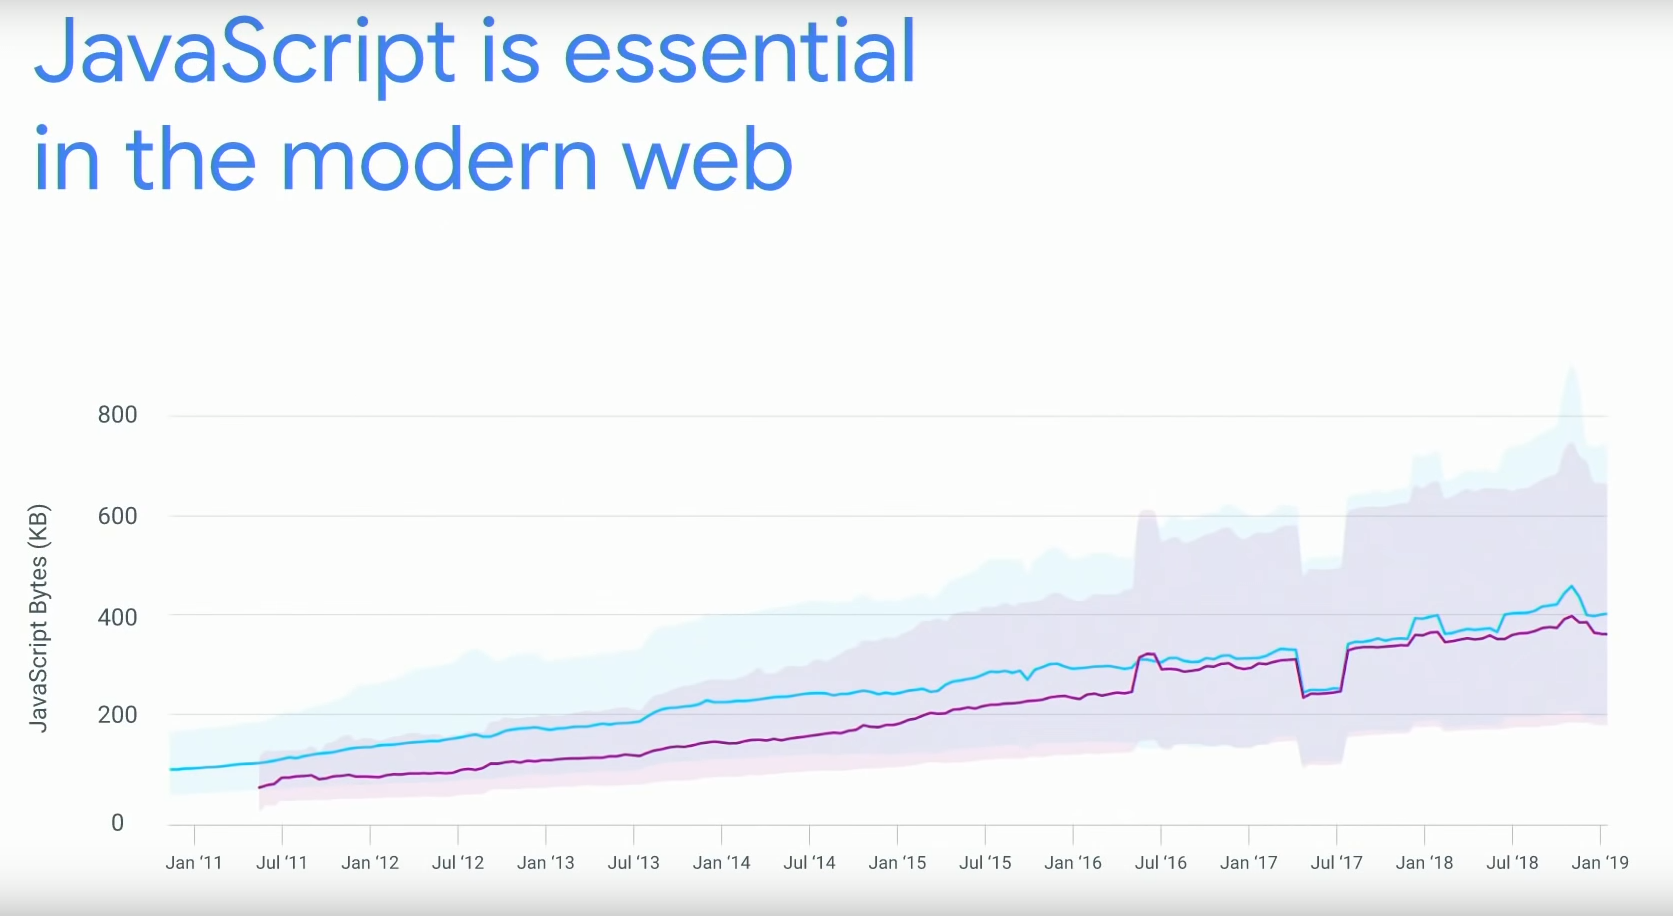
\includegraphics[width=10cm]{images/JavaScriptGoogleShips}
  \caption{JavaScript pro Webseite \cite{SearchFriendly}}
  \label{JavaScript pro Website}
\end{figure}
\\
Das Verwenden einer Single Page Anwendung 
kann sich aktuell immer noch auf die Indexierbarkeit einer Anwendung auswirken. 
Gleichzeitig besitzen noch nicht alle Suchmaschinen neue Crawler 
zum indexieren reiner clientseitigen Anwendung. 
Google berichtet, dass immer mehr JavaScript für Webseiten benötigt wird, 
wie die Abbildung \ref{JavaScript pro Website} zeigt. 
Aus diesen Gründen verbessern sie den Google Crawler weiterhin für eine bessere Indexierung von SPAs. 
In der Zukunft kann die Indexierbarkeit von CSR und SSR Anwendungen gleich sein. 
Bei der Google io 2019 sagt Google, 
dass sie sicherstellen wollen, 
dass Entwickler sich beim Erstellen von Webanwendungen auf den Inhalt konzentrieren sollen und nicht auf SEO. 
Dennoch empfiehlt Google Prerendering oder Universal Rendering, 
anstatt reine CSR, für eine gute Indexierbarkeit. \cite{WebPerfomance}
\\
\\
Da aber noch nicht alle Suchmaschinen und 
Social Media Crawler dies unterstützen ist Universal Rendering ein 
guter Workaround für eine bessere SEO und schnelle Ladezeiten für Anwender.


% -------------------------------------------------------------------------------------------------
\newpage
% Normaler LNCS Zitierstil
%\bibliographystyle{splncs}
\bibliographystyle{unsrt}
% TODO: Ändern der folgenden Zeile, damit die .bib-Datei gefunden wird
\bibliography{literatur}

\end{document}
